\section{Propuesta}
\subsection{Requerimientos Funcionales del Sistema}
Para la determinación de los requerimientos en el sistema de detección de metales pesados en el agua, se debe de tener en cuenta los siguientes:

\begin{itemize}
    \item R1. Detección Automatizada: El sistema debe ser capaz de detectar automáticamente la presencia de metales pesados específicos en muestras de agua.
    \item R2. Alerta en Tiempo Real: Debe generar alertas en tiempo real cuando los niveles de metales pesados superen los límites de seguridad establecidos.
    \item R3. Monitoreo Continuo: El sistema debe poder realizar un monitoreo continuo de la calidad del agua en ubicaciones específicas.
    \item R4. Generación de Reportes: Debe poder generar reportes detallados sobre los niveles de contaminación, incluyendo gráficos y análisis históricos.
    \item R5. Calibración y Mantenimiento: El sistema debe incluir funcionalidades para la calibración y el mantenimiento regular de los sensores de detección.
\end{itemize}

\subsection{Diagrama de Clases}
El diagrama de clases se mostrará a continuación.

\begin{figure}[h]
    \centering
    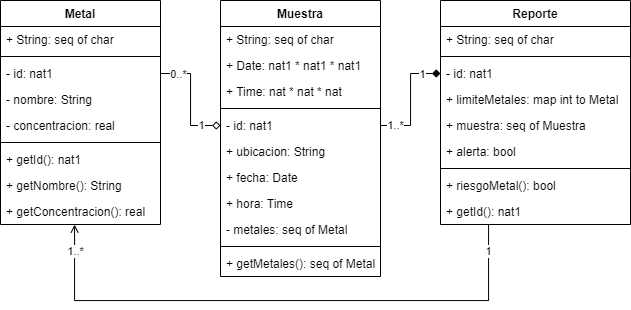
\includegraphics[width=0.5\textwidth]{Recursos/Metodos_Formales-DCL.png}
    \caption{Diagrama de Clases para la Especificación Formal y Validación de un Sistema de Detección de Metales Pesados en el Agua.}
\end{figure}

\newpage

\subsection{Sistema de Control}
El sistema de detección de metales pesados en el agua se formaliza a través de tres entidades principales: \texttt{Metal}, \texttt{Muestra}, y \texttt{Reporte}. A continuación, se describe cada uno de estos elementos.

La clase \texttt{Metal} representa cada tipo de metal presente en las muestras de agua. Los atributos de la clase son:
\begin{itemize}
    \item \textbf{id\_metal}: Identificador único para cada tipo de metal.
    \item \textbf{nombre}: Nombre descriptivo del metal (por ejemplo, mercurio o plomo) [1].
    \item \textbf{concentracion}: Concentración del metal en la muestra, expresada en unidades de partes por millón (ppm) [2], [3].
\end{itemize}

La clase \texttt{Muestra} captura la información de cada recolección de datos en el sistema:
\begin{itemize}
    \item \textbf{id\_muestra}: Identificador de la muestra.
    \item \textbf{ubicacion}: Descripción de la ubicación donde se toma la muestra.
    \item \textbf{fecha}: Fecha de recolección de la muestra.
    \item \textbf{tiempo}: Hora exacta de la recolección.
    \item \textbf{metales}: Lista de metales presentes en la muestra con sus respectivas concentraciones [4], [5].
\end{itemize}

La clase \texttt{Reporte} sintetiza los datos obtenidos de varias muestras y permite identificar riesgos:
\begin{itemize}
    \item \textbf{id\_reporte}: Identificador único del reporte generado.
    \item \textbf{limiteMetales}: Mapa que asocia el nombre del metal con su concentración límite aceptable [6].
    \item \textbf{muestra}: Lista de muestras que forman parte del reporte.
    \item \textbf{alerta}: Indica si hay alerta por sobrepasar los límites de concentración de metales [7].
\end{itemize}

El sistema emitirá una alarma en caso de que las concentraciones de los metales detectados superen los valores permitidos. La función \texttt{alertaRiesgo()} calculará si la concentración de algún metal es peligrosa para la salud humana, generando una señal de alerta [8].
